% ====================================================================================================
% SECTION 3  METHOD  (budget ~1.4 pages)
%   3.1 task (Eq. 1) | 3.2 normalized Soft F1 with document end (Eq. 2-3, Figure 2) | 3.3 evidence (Table 1, Eq. 4)
%   3.4 fusion trained for quality (Eq. 5) | 3.5 what we tried on the way
% ====================================================================================================

\section{Method}
\label{sec:method}

\subsection{Task}
\label{sec:task}
A document $X$ has words $w_1,\dots,w_{n+1}$ separated by whitespace; gap $i$ follows $w_i$. A segmentation is a vector
$y \in \{0,1\}^n$, where $y_i = 1$ means that a sentence ends after $w_i$; the end of the document is always a boundary
and is not part of $y$. With gold boundaries $g$, the true quality of $y$ is the boundary F1
\begin{equation}
  \Fone(y, g) = \frac{2\, y^{\top} g}{|y| + |g|} \qquad (\Fone = 1 \text{ if } |y| = |g| = 0),
  \label{eq:f1}
\end{equation}
with $|y| = \sum_i y_i$. An evaluator assigns a score $s(X, y)$ without reading the gold of the evaluated corpus. It is
useful to the extent that it orders candidates---within a document and across documents---as $\Fone$ does.

\subsection{Scoring a candidate against soft evidence}
\label{sec:scoring}
Suppose an evidence model gives a boundary probability $p_i \in [0,1]$ at every gap (\S\ref{sec:evidence}). We score $y$
by its F1 against $p$ used as a soft reference, counting the final boundary of the document, which every candidate and
the evidence get right, and normalize by the best score any candidate can reach:
\begin{gather}
  Q(y, p) = \frac{2\,(y^{\top} p + 1)}{|y| + \textstyle\sum_i p_i + 2}, \label{eq:q}\\
  \Qt(y, p) = \frac{Q(y, p)}{\max_{y'} Q(y', p)}, \quad
  \max_{y'} Q(y',p) = \max_{k=0,\dots,n} \frac{2\,(S_k + 1)}{k + \sum_i p_i + 2}, \label{eq:qnorm}
\end{gather}
where $S_k$ is the sum of the $k$ largest $p_i$: for a fixed number $k$ of cuts, $Q$ is largest when the cuts are at the
$k$ most probable gaps, so the maximum over all $2^n$ candidates needs only a sort. Three properties make this the right
score for our purpose.
\emph{(i) Local rewards.} Adding a cut at gap $i$ raises $Q$ exactly when $p_i > Q/2$, so a candidate is rewarded for
cutting where the evidence is confident and penalized elsewhere.
\emph{(ii) Comparability across documents.} How high a candidate can score depends on how peaked $p$ is in its document;
dividing by the attainable maximum makes $\Qt = 1$ mean ``as good as the evidence allows'' in every document. This
matters for our primary criterion, which pools candidates from all documents (\S\ref{sec:views}).
\emph{(iii) Single-sentence documents.} Without the $+1$ terms, the correct empty segmentation of a one-sentence document
has Soft F1 $= 0$ for every $p$ and is ranked last. With them it scores $2/(\sum_i p_i + 2)$ before normalization, and
$\Qt$ is close to 1 when the evidence puts little mass inside the document (e.g., $\Qt = 0.95$ when two internal gaps
have $p = 0.4$). Figure~\ref{fig:example} shows the computation on a real document.

\begin{figure}[t]
  \centering
  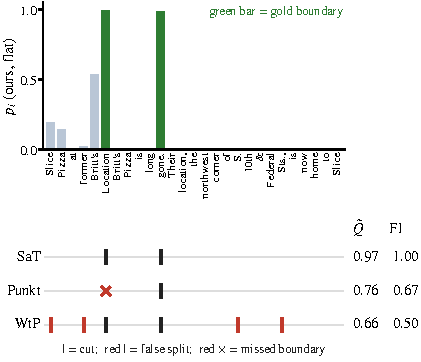
\includegraphics[width=\columnwidth]{figures/f2_example.pdf}
  \caption{A worked example: an EWT dev review whose first ``sentence'' is a title without punctuation. Bars: our flat
  evaluator's $p_i$ at each gap (labeled by the word before it). Rows: three real segmenter outputs. Punkt misses the
  unpunctuated title boundary; WtP adds false splits, two of them after the abbreviations \emph{S.} and \emph{Sts.,}.
  $\Qt$ orders the three candidates as true F1 does. Gold scores 0.97 rather than 1 because the evidence also puts
  $p = 0.54$ before the capitalized word \emph{Location}.}
  \label{fig:example}
\end{figure}

\subsection{Boundary evidence}
\label{sec:evidence}
Table~\ref{tab:evidence} lists the sources of evidence. Each produces features at every gap from the raw text alone.
The maximum-entropy probe places a \texttt{[MASK]} token at gap $i$ in a frozen \texttt{bert-base-uncased}
\citep{devlin-etal-2019-bert}---replacing a visible \emph{.?!} before the gap, inserting it otherwise---and classifies the
hidden states:
\begin{equation}
  p^{\text{probe}}_i = \sigma\big(w^{\top} [\,h^{(8)}_i;\, h^{(12)}_i;\, \ell_i\,] + b\big),
  \label{eq:probe}
\end{equation}
where $h^{(l)}_i$ is the layer-$l$ state at the mask and $\ell_i$ are insertion likelihood ratios (how much the masked
log-probabilities of the neighboring tokens change when a period is inserted). The probe is an L2-regularized logistic
regression \citep{alain-bengio-2016-understanding}. The two pretrained neural sources are the boundary probability of
SaT-12l \citep{frohmann-etal-2024-segment}, used zero-shot, and a ModernBERT-large encoder
\citep{warner-etal-2024-modernbert} that we fine-tune on GUM as a binary boundary tagger (one logit per word, binary
cross-entropy). All sources read lower-cased text except SaT-12l, which reads the original casing in the flat evaluator.

\begin{table}[t]
  \centering
  \small
  \setlength{\tabcolsep}{3pt}
  \fitbox{\begin{tabular}{@{}p{2.25cm}p{3.15cm}p{1.35cm}@{}}
    \toprule
    Source & Captures & Course topic \\
    \midrule
    Regex rules (24) & abbreviations, initials, numbering, times, quotes, distance to punctuation & regular expressions \\
    Kneser--Ney trigram (4) & $\log P(\langle/s\rangle \mid$ two left words$)$, start / continuation probabilities &
      $n$-gram LMs \\
    Probe on BERT (1) & Eq.~\ref{eq:probe}: punctuation vs.\ sentence boundary in context & MaxEnt / logistic reg. \\
    SaT-12l (1) & pretrained boundary model, zero-shot & --- \\
    ModernBERT tagger (1) & boundary tagger fine-tuned on GUM & sequence labeling \\
    Paragraph flag (1) & newline at the gap (layout only) & --- \\
    \bottomrule
  \end{tabular}}
  \caption{Evidence sources (number of features in parentheses). Rules and $n$-gram counts are fitted on GUM train only;
  details in App.~\ref{app:method}.}
  \label{tab:evidence}
\end{table}

\subsection{Fusion trained for quality}
\label{sec:fusion}
The features of gap $i$ are stacked into $x_i$ (31 dimensions; 32 with the paragraph flag) and fused by a logistic model
$p_i = \sigma(\theta^{\top} x_i)$. A plain boundary classifier treats all gaps alike, although most gaps are easy and only
the few where segmenters disagree decide which candidate is better. We therefore fit $\theta$ on GUM train for both
boundary accuracy and score quality:
\begin{gather}
  J(\theta) = \frac{L_Q(\theta)}{L_Q(\theta_0)} + \frac{L_B(\theta) + \frac{\lambda}{2}\lVert\theta\rVert^2}{L_B(\theta_0)},
  \label{eq:objective}\\
  L_Q(\theta) = \frac{1}{|\mathcal{I}|}\sum_{(d,s)\in\mathcal{I}} \big(\Qt^{0}(y_{ds}, p_\theta) - \Fone(y_{ds}, g_d)\big)^2,
  \nonumber
\end{gather}
where $\mathcal{I}$ contains every training document $d$ paired with the output $y_{ds}$ of each of the four segmenters
$s$, $L_B$ is the mean binary cross-entropy of $p_\theta$ against gold over all gaps, and $\theta_0$ is the
boundary-only solution (L2 logistic regression, $\lambda = 10^{-3}$), which also initializes L-BFGS
\citep{liu-nocedal-1989-limited}; gradients pass through the sort in Eq.~\ref{eq:qnorm}. As implemented, the training
objective uses the normalized Soft F1 \emph{without} the document-end term ($\Qt^0$), while evaluation uses $\Qt$. No GUM
document is a single sentence; there the two scores differ per item by 0.001--0.002 on average (at most 0.04) and give the
same agreement with true quality to three decimals (0.903 flat, 0.948 with paragraphs), so we kept the frozen models.
In a controlled comparison on GUM (same features, folds and items), this objective beats boundary-only training, whereas
a quality loss alone or a post-hoc quality-estimation regression over the four seen segmenters does not, and both
degrade when a segmenter is held out (App.~\ref{app:objective}).

We fit two evaluators: \emph{flat}, for plain text (the default), and \emph{layout}, which also sees paragraph breaks
(\S\ref{sec:data}); the layout evaluator is lower-cased throughout and adds the paragraph flag.

\subsection{What we tried on the way}
\label{sec:tried}
Our first evaluators used the Platt-calibrated BERT probability of a terminal punctuation mark at the gap
(\emph{PuncEv}), and then the probe alone; each was frozen and tested once on EWT test. A semi-Markov sentence-length
prior on top of the evidence did not help on any corpus; letting BERT see the candidate's own boundaries made the
evidence agree with the candidate's errors; post-hoc quality regression learned the four seen segmenters rather than
quality; and a left-to-right LLM (Qwen) gave evidence that normalization could not make comparable across documents.
App.~\ref{app:prelim}--\ref{app:method} give details; the development ladder from the probe to the final evaluator is in
App.~\ref{app:ladder}.
